\chapter{Ứng dụng Zero Trust bảo mật hệ thống Microservices}

%==============================================================================
% 2.1 BÀI TOÁN BẢO MẬT ĐẶC THÙ
%==============================================================================
\section{Bài toán bảo mật đặc thù của hệ thống Microservices}

Kiến trúc Microservices phân rã ứng dụng thành nhiều dịch vụ độc lập, mỗi dịch vụ đảm nhiệm một chức năng nghiệp vụ riêng và giao tiếp với nhau thông qua mạng \parencite{lewis_fowler_2014}. Cách tiếp cận này giúp tăng khả năng mở rộng, triển khai độc lập và nâng cao tính linh hoạt trong quá trình phát triển phần mềm. Tuy nhiên, việc gia tăng số lượng thành phần phân tán cũng làm mở rộng đáng kể bề mặt tấn công của hệ thống so với mô hình ứng dụng nguyên khối truyền thống.

Trong thực tế, các hệ thống Microservices thường được triển khai trên nền tảng điều phối container như Kubernetes nhằm tự động hóa quá trình vận hành, mở rộng và phục hồi dịch vụ. Mặc dù mang lại nhiều lợi ích về mặt quản trị hạ tầng, môi trường này đồng thời tạo ra các thách thức bảo mật mới liên quan đến định danh thực thể, bảo vệ lưu lượng nội bộ, quản lý thông tin xác thực và giám sát hành vi tại thời điểm chạy.

Tiêu chuẩn NIST SP 800-204 chỉ ra rằng môi trường Microservices làm gia tăng đáng kể mức độ phụ thuộc vào giao tiếp mạng giữa các dịch vụ, khiến giả định về một mạng nội bộ đáng tin cậy không còn phù hợp \parencite{nist800204_microservices}. Trong bối cảnh đó, các cơ chế bảo mật tập trung tại biên mạng không còn đủ khả năng bảo vệ hệ thống trước các cuộc tấn công xuất phát từ bên trong hoặc các hành vi di chuyển ngang giữa các thành phần đã bị xâm phạm.

Do đó, trước khi xây dựng kiến trúc Zero Trust cho hệ thống Microservices, cần phân tích các thách thức bảo mật đặc thù phát sinh từ đặc tính phân tán, môi trường điều phối Kubernetes và chuỗi cung ứng phần mềm. Kết quả phân tích này là cơ sở để xác định các yêu cầu kỹ thuật mà kiến trúc đề xuất cần đáp ứng.


%------------------------------------------------------------------------------
\subsection{Thách thức định danh và quản lý thông tin xác thực}
%------------------------------------------------------------------------------

Trong kiến trúc Microservices, mỗi dịch vụ cần xác thực danh tính của các dịch vụ khác trước khi trao đổi dữ liệu hoặc truy cập tài nguyên. Quá trình này làm phát sinh số lượng lớn thông tin xác thực như khóa API, chứng chỉ số, mật khẩu dịch vụ hoặc mã truy cập tạm thời. Khi quy mô hệ thống tăng lên, việc quản lý các thông tin này trở nên phức tạp và dễ dẫn đến tình trạng phân tán thông tin xác thực trên nhiều thành phần khác nhau.

Một thực tiễn phổ biến nhưng tiềm ẩn nhiều rủi ro là lưu trữ trực tiếp thông tin xác thực trong mã nguồn, tệp cấu hình hoặc biến môi trường. Nếu một thành phần bị xâm phạm, tác nhân tấn công có thể thu thập các thông tin này để mở rộng phạm vi truy cập sang các dịch vụ khác trong hệ thống. Trong môi trường Microservices, một thông tin xác thực bị lộ thường không chỉ ảnh hưởng đến một dịch vụ đơn lẻ mà còn có thể tác động đến toàn bộ chuỗi phụ thuộc giữa các dịch vụ.

Bên cạnh đó, các hệ thống quản lý bí mật tập trung cũng phải đối mặt với bài toán Secret Zero \parencite{vault_docs}. Đây là vấn đề xác thực ban đầu đối với chính hệ thống quản lý bí mật. Nếu thông tin xác thực gốc dùng để truy cập kho bí mật bị lộ hoặc bị đánh cắp, toàn bộ cơ chế bảo vệ phía sau có thể bị vô hiệu hóa.

Những thách thức này cho thấy hệ thống cần một cơ chế định danh độc lập với địa chỉ mạng, đồng thời hỗ trợ cấp phát, luân chuyển và thu hồi thông tin xác thực một cách tự động trong suốt vòng đời hoạt động của thực thể.

%------------------------------------------------------------------------------
\subsection{Thách thức từ môi trường điều phối Kubernetes}
%------------------------------------------------------------------------------

Kubernetes cung cấp khả năng tự động triển khai, mở rộng và phục hồi ứng dụng, tuy nhiên các đặc tính này đồng thời tạo ra nhiều yêu cầu bảo mật mới so với môi trường triển khai truyền thống.

Trước hết, các Pod được tạo mới, thay thế hoặc thu hồi liên tục trong quá trình vận hành. Tính chất ngắn hạn này khiến địa chỉ IP và vị trí thực thi của các khối lượng công việc thay đổi thường xuyên \parencite{k8s_pod_lifecycle}. Do đó, việc sử dụng địa chỉ mạng như một thuộc tính nhận dạng trở nên kém hiệu quả, đặc biệt trong các cơ chế kiểm soát truy cập hoặc thực thi chính sách bảo mật.

Bên cạnh đó, Kubernetes sử dụng cơ chế phân quyền dựa trên RBAC để kiểm soát quyền truy cập vào tài nguyên của cụm. Việc cấu hình quyền hạn không phù hợp cho người dùng, ServiceAccount hoặc thành phần tự động hóa có thể tạo điều kiện cho tác nhân tấn công mở rộng phạm vi kiểm soát sau khi xâm nhập thành công \parencite{kubernetes_docs}. Các quyền có mức ảnh hưởng cao như tạo Pod đặc quyền, gắn ServiceAccount hoặc thao tác với tài nguyên điều phối có thể trở thành con đường leo thang đặc quyền trong cụm.

Những đặc điểm trên đặt ra yêu cầu phải tách biệt khái niệm định danh khỏi thông tin hạ tầng động, đồng thời áp dụng cơ chế ủy quyền tập trung và nhất quán trên toàn bộ môi trường điều phối.

%------------------------------------------------------------------------------
\subsection{Thách thức bảo mật mạng nội bộ}
%------------------------------------------------------------------------------

Khác với kiến trúc nguyên khối, phần lớn các tương tác trong hệ thống Microservices được thực hiện thông qua mạng nội bộ giữa các dịch vụ. Điều này làm gia tăng đáng kể lưu lượng East-West và biến mạng nội bộ thành một trong những bề mặt tấn công quan trọng nhất của hệ thống.

Trong trường hợp một dịch vụ bị thỏa hiệp, tác nhân tấn công có thể lợi dụng các kết nối hợp lệ đã tồn tại để thực hiện trinh sát, thu thập thông tin hoặc di chuyển ngang sang các thành phần khác. Mức độ rủi ro càng gia tăng khi các dịch vụ mặc định tin cậy lẫn nhau chỉ vì cùng nằm trong một cụm Kubernetes hoặc cùng thuộc một vùng mạng.

Một giải pháp thường được áp dụng là mã hóa toàn bộ lưu lượng nội bộ bằng cơ chế xác thực hai chiều. Tuy nhiên, việc bổ sung các lớp kiểm soát bảo mật trên đường truyền cũng có thể làm gia tăng chi phí xử lý và độ trễ truyền thông. Do đó, hệ thống cần đạt được sự cân bằng giữa yêu cầu bảo mật, khả năng mở rộng và hiệu năng vận hành.

Những thách thức này cho thấy việc bảo vệ mạng nội bộ không chỉ dừng ở mã hóa lưu lượng mà còn đòi hỏi khả năng xác thực danh tính, thực thi chính sách truy cập và kiểm soát giao tiếp giữa các thực thể ở mức chi tiết.

%------------------------------------------------------------------------------
\subsection{Thách thức giám sát và bảo vệ tại thời điểm chạy}
%------------------------------------------------------------------------------

Các biện pháp bảo mật truyền thống như kiểm tra mã nguồn, quét lỗ hổng hoặc đánh giá cấu hình chủ yếu được thực hiện trước khi hệ thống đi vào vận hành. Mặc dù giúp giảm thiểu nhiều nguy cơ bảo mật, các biện pháp này không đủ khả năng phát hiện những hành vi phát sinh trong quá trình thực thi.

Trong thực tế, tác nhân tấn công có thể khai thác các lỗ hổng chưa được công bố, thực thi mã độc trực tiếp trong bộ nhớ hoặc sử dụng các lời gọi hệ thống bất thường để vượt qua các cơ chế bảo vệ hiện có. Các hoạt động này thường không để lại dấu hiệu rõ ràng trên mã nguồn hoặc container image đã được kiểm tra trước đó.

Bên cạnh đó, các container trên cùng một nút tính toán chia sẻ chung nhân hệ điều hành. Những lỗ hổng tại lớp runtime hoặc nhân hệ điều hành có thể bị khai thác để thực hiện các kỹ thuật vượt thoát container và chiếm quyền kiểm soát máy chủ lưu trữ \parencite{cve_2024_21626,cve_2022_0847}.

Do đó, hệ thống cần khả năng quan sát liên tục đối với các hoạt động diễn ra tại thời điểm chạy, bao gồm hành vi tiến trình, tương tác mạng và các lời gọi hệ thống quan trọng. Dữ liệu quan sát được phải có khả năng hỗ trợ phát hiện bất thường và cung cấp ngữ cảnh cho quá trình ra quyết định bảo mật.

%------------------------------------------------------------------------------
\subsection{Thách thức từ chuỗi cung ứng phần mềm}
%------------------------------------------------------------------------------

Mỗi khối lượng công việc triển khai trong Kubernetes thường được xây dựng từ nhiều thành phần phần mềm khác nhau như hệ điều hành nền, thư viện phụ thuộc, container image và các gói mã nguồn từ bên thứ ba. Điều này khiến chuỗi cung ứng phần mềm trở thành một mục tiêu hấp dẫn đối với tác nhân tấn công.

Một container image chứa mã độc, thư viện bị cài cắm hoặc được phát hành từ nguồn không đáng tin cậy có thể đưa mã thực thi độc hại trực tiếp vào môi trường sản xuất mà không cần khai thác bất kỳ lỗ hổng nào trên hệ thống đang vận hành. Các cuộc tấn công vào chuỗi cung ứng phần mềm trong những năm gần đây cho thấy việc bảo vệ môi trường thực thi là chưa đủ nếu nguồn gốc của khối lượng công việc không được xác minh.

Do đó, ngoài việc kiểm tra lỗ hổng bảo mật, hệ thống cần có khả năng xác thực nguồn gốc, tính toàn vẹn và trạng thái phê duyệt của các thành phần trước khi cho phép triển khai vào môi trường vận hành.

%------------------------------------------------------------------------------
\subsection{Phân tích bề mặt tấn công theo mô hình MITRE ATT\&CK}
%------------------------------------------------------------------------------

Các thách thức bảo mật đã phân tích ở các mục trước phản ánh những đặc điểm nội tại của kiến trúc Microservices và môi trường Kubernetes. Tuy nhiên, để đánh giá mức độ liên hệ giữa các thách thức này với các mối đe dọa trong thực tế, cần đối chiếu chúng với một mô hình phân tích tấn công có tính hệ thống và được thừa nhận rộng rãi.

Trong phạm vi đồ án, khung MITRE ATT\&CK dành cho Container được sử dụng làm cơ sở tham chiếu \parencite{mitre_containers}. Đây là cơ sở tri thức mô tả hành vi của tác nhân tấn công thông qua tập hợp các chiến thuật và kỹ thuật đã được quan sát trong thực tế. Đối với môi trường container và Kubernetes, MITRE ATT\&CK cung cấp một góc nhìn toàn diện về chuỗi tấn công, từ giai đoạn xâm nhập ban đầu, thiết lập chỗ đứng trong hệ thống cho đến các hoạt động hậu khai thác như leo thang đặc quyền, di chuyển ngang và gây tác động lên tài nguyên.

Việc đối chiếu với MITRE ATT\&CK không nhằm liệt kê đầy đủ mọi kỹ thuật tấn công có thể xảy ra, mà tập trung xác định những thành phần hệ thống thường xuyên trở thành mục tiêu trong môi trường Microservices. Kết quả phân tích cho phép đánh giá liệu các thách thức đã được nhận diện trước đó có phản ánh đúng thực tiễn tấn công hay không, đồng thời làm cơ sở để xác định các yêu cầu kỹ thuật đối với kiến trúc Zero Trust được đề xuất.

Hình \ref{fig:mitre_containers} minh họa các chiến thuật và kỹ thuật tấn công phổ biến đối với môi trường container theo khung MITRE ATT\&CK.

\begin{figure}[H]
    \centering
    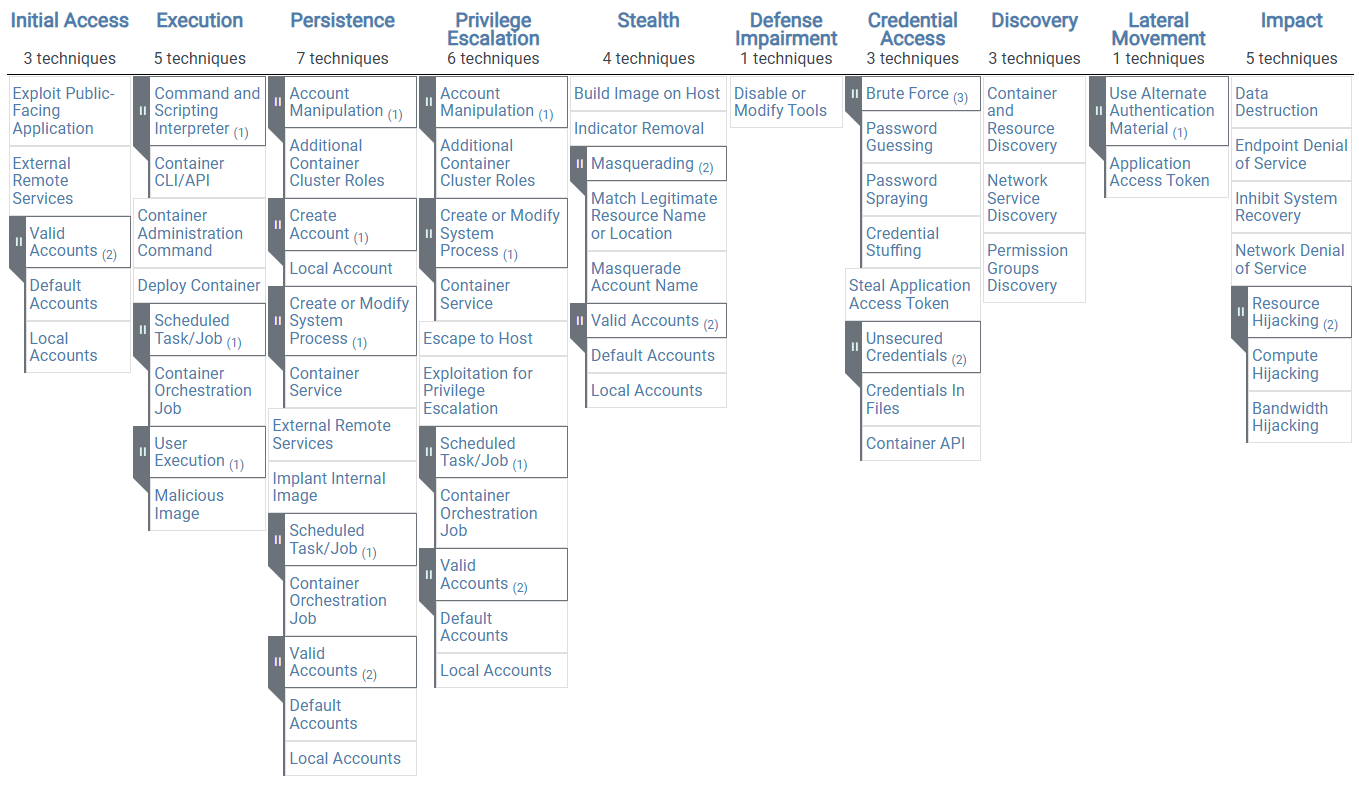
\includegraphics[width=\textwidth]{images/mitre_attack_containers.png}
    \caption[Các kỹ thuật tấn công vào môi trường Container]{Các chiến thuật và kỹ thuật tấn công đối với môi trường Container theo khung MITRE ATT\&CK \parencite{mitre_containers}.}
    \label{fig:mitre_containers}
\end{figure}

Để thuận tiện cho việc phân tích, các kỹ thuật tiêu biểu được nhóm thành hai giai đoạn chính gồm giai đoạn xâm nhập và thiết lập chỗ đứng trong hệ thống, cùng giai đoạn hậu khai thác và mở rộng phạm vi ảnh hưởng.

\begin{table}[H]
\centering
\caption{Các kỹ thuật MITRE ATT\&CK liên quan đến giai đoạn xâm nhập và thiết lập chỗ đứng}
\label{tab:mitre_phase1}
\renewcommand{\arraystretch}{1.3}
\begin{tabularx}{\textwidth}{|p{3.5cm}|X|p{4.5cm}|}
\hline
\textbf{Chiến thuật} &
\textbf{Kỹ thuật tiêu biểu} &
\textbf{Thách thức liên quan} \\
\hline

Xâm nhập ban đầu &
Khai thác ứng dụng công khai (T1190); Lạm dụng tài khoản hợp lệ (T1078) &
Định danh và quản lý thông tin xác thực \\
\hline

Thực thi &
Triển khai image chứa mã độc (T1610); Thực thi lệnh thông qua API điều phối (T1609) &
Chuỗi cung ứng phần mềm; Môi trường Kubernetes \\
\hline

Duy trì truy cập &
Tạo tác vụ định kỳ (T1053); Triển khai container chạy nền (T1525) &
Môi trường Kubernetes; Giám sát thời gian chạy \\
\hline

Ẩn mình &
Trá hình tiến trình (T1036); Xóa dấu vết hoạt động (T1070) &
Khả năng quan sát và giám sát thời gian chạy \\
\hline

Vô hiệu hóa phòng thủ &
Sửa đổi hoặc vô hiệu hóa cơ chế bảo vệ (T1562) &
Giám sát thời gian chạy; Thực thi chính sách bảo mật \\
\hline

\end{tabularx}
\end{table}

\begin{table}[H]
\centering
\caption{Các kỹ thuật MITRE ATT\&CK liên quan đến giai đoạn hậu khai thác}
\label{tab:mitre_phase2}
\renewcommand{\arraystretch}{1.3}
\begin{tabularx}{\textwidth}{|p{3.5cm}|X|p{4.5cm}|}
\hline
\textbf{Chiến thuật} &
\textbf{Kỹ thuật tiêu biểu} &
\textbf{Thách thức liên quan} \\
\hline

Leo thang đặc quyền &
Vượt thoát container hoặc khai thác đặc quyền máy chủ (T1611) &
Môi trường Kubernetes; Bảo vệ thời gian chạy \\
\hline

Truy cập thông tin nhạy cảm &
Thu thập thông tin xác thực từ tệp cấu hình hoặc biến môi trường (T1552) &
Định danh và quản lý thông tin xác thực \\
\hline

Trinh sát &
Dò quét dịch vụ và tài nguyên nội bộ (T1046, T1613) &
Bảo mật mạng nội bộ \\
\hline

Di chuyển ngang &
Lợi dụng dịch vụ nội bộ hoặc tái sử dụng thông tin xác thực (T1021) &
Bảo mật mạng nội bộ; Định danh và ủy quyền \\
\hline

Tác động &
Chiếm dụng tài nguyên điện toán (T1496); Tấn công từ chối dịch vụ (T1498) &
Khả năng chống chịu và bảo vệ tài nguyên hệ thống \\
\hline

\end{tabularx}
\end{table}


Từ kết quả phân tích, đồ án xác định bốn yêu cầu kỹ thuật cốt lõi làm cơ sở cho việc thiết kế kiến trúc Zero Trust trong các chương tiếp theo.

\begin{enumerate}[itemsep=6pt, parsep=0pt]

\item \textbf{Thiết lập định danh độc lập với hạ tầng mạng}

Trong môi trường Kubernetes, các thực thể có tính động cao, địa chỉ IP và vị trí thực thi thay đổi liên tục trong quá trình vận hành. Do đó, hệ thống cần một cơ chế định danh ổn định, có khả năng xác minh bằng mật mã học và không phụ thuộc vào thông tin định tuyến hoặc vị trí triển khai của thực thể.

\item \textbf{Quản lý vòng đời thông tin xác thực}

Thông tin xác thực cần được cấp phát, sử dụng, luân chuyển và thu hồi theo vòng đời hoạt động của thực thể. Kiến trúc phải hạn chế việc lưu trữ tĩnh các bí mật trong mã nguồn hoặc cấu hình, đồng thời bảo đảm khả năng phân phối thông tin xác thực một cách tự động và có kiểm soát.

\item \textbf{Thực thi chính sách truy cập phân tán và nhất quán}

Các quyết định truy cập không thể phụ thuộc vào một điểm kiểm soát duy nhất. Hệ thống cần khả năng thực thi chính sách tại nhiều vị trí khác nhau như lớp mạng, môi trường thực thi, thành phần ứng dụng và nền tảng điều phối, đồng thời duy trì tính nhất quán trong quá trình đánh giá và cấp quyền.

\item \textbf{Ra quyết định dựa trên ngữ cảnh và khả năng quan sát}

Việc cấp quyền truy cập cần dựa trên nhiều yếu tố hơn là danh tính của thực thể. Kiến trúc phải có khả năng thu thập dữ liệu quan sát từ môi trường vận hành, liên kết dữ liệu này với định danh tương ứng và sử dụng chúng làm đầu vào cho quá trình đánh giá rủi ro và thực thi chính sách.

\end{enumerate}

Bốn yêu cầu kỹ thuật trên phản ánh trực tiếp các thách thức bảo mật đã được nhận diện trong môi trường Microservices. Đây cũng là cơ sở để xây dựng kiến trúc logic Zero Trust được trình bày trong các mục tiếp theo của chương.


%==============================================================================
% 2.2 KIẾN TRÚC ZERO TRUST ĐỀ XUẤT
%==============================================================================
\section{Kiến trúc Zero Trust đề xuất}

Kiến trúc đề xuất hiện thực hóa ba vai trò logic của NIST SP 800-207 ---
Điểm cung cấp thông tin (PIP), Điểm quyết định chính sách (PDP) và Điểm
thực thi chính sách (PEP) --- thành năm thành phần chức năng, phân tách
theo tần suất cập nhật và vị trí trong luồng xử lý yêu cầu truy cập
\parencite{nist800207}. Thành phần 1 và Thành phần 2 đóng vai trò PIP với
hai loại ngữ cảnh khác nhau về tần suất cập nhật; Thành phần 3 là PDP;
Thành phần 4 là PEP; Thành phần 5 là PIP telemetry đóng vòng phản hồi về
Thành phần 3.

Luồng xử lý một yêu cầu truy cập diễn ra tuần tự: xác thực định danh
của thực thể, đánh giá trạng thái bảo mật hiện tại, ra quyết định cấp
quyền, thực thi quyết định tại các điểm kiểm soát, và ghi nhận sự kiện
để cập nhật ngữ cảnh cho vòng đánh giá tiếp theo.

\begin{figure}[H]
\centering
\begin{tikzpicture}[
  font=\footnotesize\sffamily,
  blk/.style={draw, rounded corners=3pt, minimum height=13mm,
               text width=12.5cm, align=left, inner sep=6pt, line width=0.6pt},
  s1/.style={blk, fill=blue!7,    draw=blue!50},
  s2/.style={blk, fill=cyan!7,    draw=cyan!50},
  s3/.style={blk, fill=orange!9,  draw=orange!60},
  s4/.style={blk, fill=green!8,   draw=green!50},
  s5/.style={blk, fill=violet!7,  draw=violet!50},
  lbl/.style={font=\scriptsize\sffamily\itshape, text=gray!65}
]

\node[s1] (s1) at (0,12.0) {
  \textbf{Thành phần 1 — Định danh và Xác thực}
  \hfill \lbl{PIP · cập nhật theo TTL chứng chỉ}\\[3pt]
  Cấp và xác minh định danh mật mã học cho mọi thực thể trước khi yêu cầu
  được xem xét. Người dùng xác thực qua giao thức OIDC và nhận mã truy cập
  ngắn hạn. Mỗi workload được cấp chứng chỉ định danh X.509 theo chuẩn
  SPIFFE, có thời gian sống ngắn và tự động gia hạn, thay thế địa chỉ IP
  làm căn cứ nhận dạng.};

\node[s2] (s2) at (0, 8.8) {
  \textbf{Thành phần 2 — Đánh giá tư thế bảo mật}
  \hfill \lbl{PIP · cập nhật theo batch và sự kiện}\\[3pt]
  Thu thập và duy trì ngữ cảnh bảo mật động của từng workload để cung cấp
  cho Thành phần 3. Bao gồm quét lỗ hổng phần mềm định kỳ trên image đang
  chạy, kiểm tra tuân thủ cấu hình và đồng bộ danh sách địa chỉ độc hại
  từ nguồn tình báo bên ngoài. Thành phần này không trực tiếp thực thi
  chính sách --- toàn bộ dữ liệu được chuyển sang Thành phần 3 để ra
  quyết định.};

\node[s3] (s3) at (0, 5.5) {
  \textbf{Thành phần 3 — Ra quyết định và Phân phối chính sách}
  \hfill \lbl{PDP · PE + PA}\\[3pt]
  Nhận định danh từ Thành phần 1 và ngữ cảnh từ Thành phần 2, áp dụng
  thuật toán đánh giá rủi ro đa chiều để xác định mức độ tin cậy và hành
  động phản hồi phù hợp. Đồng thời điều phối cấp phát thông tin xác thực
  tạm thời theo cơ chế JIT cho workload được phê duyệt --- việc tiêm thông
  tin xác thực vào môi trường thực thi được thực hiện bởi Thành phần 4.};

\node[s4] (s4) at (0, 2.3) {
  \textbf{Thành phần 4 — Thực thi chính sách}
  \hfill \lbl{PEP · biên · mạng · admission · runtime}\\[3pt]
  Thực thi quyết định từ Thành phần 3 tại bốn vị trí độc lập nhau. Tại
  biên hệ thống: kiểm tra hiệu lực mã truy cập. Tại mạng nội bộ: áp dụng
  chính sách từ chối mặc định, chỉ cho phép luồng được khai báo tường
  minh kết hợp xác thực định danh mTLS. Tại cổng nạp: kiểm tra tính toàn
  vẹn và nguồn gốc image. Tại runtime: giám sát và kiểm soát lời gọi hệ
  thống bất thường ở tầng nhân.};

\node[s5] (s5) at (0,-0.6) {
  \textbf{Thành phần 5 — Quan sát và Phản hồi thích ứng}
  \hfill \lbl{PIP · telemetry thời gian thực → Thành phần 3}\\[3pt]
  Thu thập toàn bộ sự kiện từ bốn thành phần trên và đưa trở lại Thành
  phần 3 làm ngữ cảnh cho vòng đánh giá tiếp theo. Mỗi bản ghi sự kiện
  mạng được gắn định danh thực thể thay vì địa chỉ IP. Khi phát hiện tín
  hiệu bất thường, Thành phần 3 cập nhật đánh giá rủi ro và phân phối
  chính sách mới xuống Thành phần 4 mà không cần can thiệp thủ công.};

\foreach \from/\to in {s1/s2, s2/s3, s3/s4, s4/s5}
  \draw[->, >=Latex, gray!55, line width=0.7pt] (\from) -- (\to);

\draw[->, >=Latex, dashed, gray!50, line width=0.7pt]
  (s5.east) -- ++(1.6,0) |-
  node[pos=0.25, right, font=\scriptsize\sffamily, text=gray!60,
       align=left, xshift=2pt] {Cập nhật ngữ cảnh\\cho vòng đánh giá tiếp theo}
  (s3.east);

\end{tikzpicture}
\caption{Năm thành phần chức năng của kiến trúc Zero Trust đề xuất và ánh
         xạ vào ba vai trò logic NIST SP 800-207}
\label{fig:zta_five_components}
\end{figure}

%------------------------------------------------------------------------------
\subsection{Thành phần 1 — Định danh và Xác thực}
%------------------------------------------------------------------------------

\textbf{Vai trò:} Cung cấp định danh mật mã học cho mọi thực thể trong hệ thống, thay thế địa chỉ IP làm căn cứ kiểm soát truy cập. Đây là đầu vào bắt buộc cho Thành phần 3 --- không có định danh hợp lệ thì không có quyết định cấp quyền.

\textbf{Định danh người dùng:} Người dùng xác thực qua giao thức OIDC và nhận mã truy cập dạng JWT có thời gian sống ngắn. JWT mang theo các thuộc tính phân quyền phục vụ quá trình đánh giá ở Thành phần 3.

\textbf{Định danh workload:} Mỗi workload khi khởi tạo được cấp một chứng chỉ X.509 SVID theo chuẩn SPIFFE \parencite{spiffe_spec}. Chứng chỉ có thời gian sống rất ngắn, tự động gia hạn và không phụ thuộc vào địa chỉ IP hay cấu hình mạng. Workload sử dụng SVID để xác thực lẫn nhau qua mTLS trên mạng nội bộ.

\textbf{Chế độ lỗi:} Nếu dịch vụ cấp chứng chỉ không phản hồi, các SVID hiện có vẫn hợp lệ đến hết TTL. Workload mới không thể khởi động khi chưa có SVID hợp lệ --- đây là hành vi từ chối an toàn có chủ đích.

%------------------------------------------------------------------------------
\subsection{Thành phần 2 — Đánh giá tư thế bảo mật}
%------------------------------------------------------------------------------

\textbf{Vai trò:} Thu thập và duy trì ngữ cảnh bảo mật động của từng workload để Thành phần 3 có đủ thông tin ra quyết định. Thành phần 2 không thực thi chính sách --- ranh giới này đảm bảo tính tách biệt giữa thu thập dữ liệu và ra quyết định.

\textbf{Đánh giá lỗ hổng:} Quét định kỳ các image đang chạy và sinh báo cáo lỗ hổng dưới dạng tài nguyên Kubernetes. Khi CVE mới được công bố, báo cáo cập nhật tự động mà không cần triển khai lại workload.

\textbf{Kiểm tra tuân thủ cấu hình:} Đánh giá tài nguyên Kubernetes theo tập hợp ràng buộc định nghĩa trước --- nhãn bắt buộc, cấu hình bảo mật Pod, quyền hạn tối thiểu. Kết quả được chuyển sang Thành phần 3 làm một trong các yếu tố tính điểm rủi ro.

\textbf{Tình báo đe dọa:} Đồng bộ định kỳ danh sách địa chỉ IP và tên miền độc hại từ nguồn bên ngoài. Dữ liệu này được Thành phần 3 sử dụng để phát hiện lưu lượng đến các đích đã biết là độc hại.

\textbf{Chế độ lỗi:} Nếu quá trình quét gián đoạn, kết quả cũ được giữ nguyên với trạng thái lỗi thời. Thành phần 3 tính điểm dựa trên dữ liệu này với mức tin cậy thấp hơn thay vì tự động chặn.

%------------------------------------------------------------------------------
\subsection{Thành phần 3 — Ra quyết định và Phân phối chính sách}
%------------------------------------------------------------------------------

\textbf{Vai trò:} Nhận định danh từ Thành phần 1 và ngữ cảnh từ Thành phần 2 và Thành phần 5, tính toán mức độ rủi ro, ra quyết định và phân phối quyết định đó xuống Thành phần 4. Đây là thành phần duy nhất có thể thay đổi trạng thái kiểm soát truy cập của một workload.

\textbf{Đánh giá rủi ro đa chiều:} Thay vì gán điểm phạt tuyến tính theo mức độ nghiêm trọng của lỗ hổng, Động cơ chính sách đánh giá rủi ro theo ba chiều độc lập: mức độ nghiêm trọng của lỗ hổng, khả năng khai thác qua mạng và phân cấp dịch vụ. Cơ chế đánh giá và ma trận phản hồi được trình bày chi tiết tại Mục~\ref{sec:risk_model}.

\textbf{Phân phối chính sách:} Bộ điều phối chính sách cập nhật nhãn phân cấp rủi ro trên workload và đồng bộ chính sách mạng tương ứng xuống Thành phần 4. Các điểm thực thi đối chiếu nhãn này khi xử lý lưu lượng, không cần kết nối trực tiếp về Thành phần 3 cho mỗi yêu cầu.

\textbf{Cấp phát thông tin xác thực động:} Thành phần 3 phê duyệt yêu cầu cấp thông tin xác thực tạm thời theo cơ chế JIT. Khi một workload được phê duyệt, hệ thống cấp tài khoản ngẫu nhiên với TTL ngắn. Việc tiêm thông tin xác thực vào môi trường thực thi của Pod được thực hiện bởi cơ chế sidecar thuộc Thành phần 4.

\textbf{Chế độ lỗi:} Nếu Thành phần 3 không phản hồi, các điểm thực thi ở Thành phần 4 giữ nguyên chính sách cuối cùng nhận được --- không tự động mở thêm quyền.

%------------------------------------------------------------------------------
\subsection{Thành phần 4 — Thực thi chính sách}
%------------------------------------------------------------------------------

\textbf{Vai trò:} Thực thi quyết định từ Thành phần 3 tại bốn vị trí độc lập nhau. Không điểm thực thi nào trong Thành phần 4 tự ra quyết định --- tất cả đối chiếu với chính sách được phân phối từ Thành phần 3.

\textbf{Kiểm soát biên:} Tại cửa ngõ hệ thống, mọi yêu cầu từ bên ngoài phải mang mã truy cập hợp lệ. Chính sách kiểm tra được đánh giá theo ngữ cảnh yêu cầu trước khi cho phép đi tiếp vào cluster.

\textbf{Kiểm soát mạng nội bộ:} Áp dụng chính sách từ chối mặc định trên toàn bộ lưu lượng East-West. Luồng giao tiếp giữa các workload chỉ được phép khi có khai báo tường minh trong chính sách mạng, kết hợp với xác thực định danh mTLS. Chính sách gắn theo nhãn workload, không theo địa chỉ IP --- tự động theo workload khi được tái lập lịch sang Node khác.

\textbf{Kiểm soát cổng nạp:} Mọi tài nguyên được đánh giá trước khi được chấp nhận vào cluster. Image phải có chữ ký số từ chuỗi cung ứng tin cậy. Hỗ trợ chế độ ghi nhận trước khi chuyển sang chặn tuyệt đối, cho phép tinh chỉnh cấu hình mà không gây gián đoạn dịch vụ.

\textbf{Kiểm soát runtime:} Giám sát lời gọi hệ thống tại tầng nhân thông qua cơ chế eBPF. Hoạt động hoàn toàn độc lập với không gian người dùng của Pod --- workload không thể can thiệp vào quá trình giám sát của chính nó. Hành vi bất thường được ghi nhận hoặc ngắt tùy theo chính sách cấu hình.

\textbf{Chế độ lỗi:} Nếu một điểm thực thi mất kết nối với Thành phần 3, nó giữ nguyên chính sách cuối cùng nhận được. Các điểm thực thi còn lại vẫn hoạt động độc lập nhau.

%------------------------------------------------------------------------------
\subsection{Thành phần 5 — Quan sát và Phản hồi thích ứng}
%------------------------------------------------------------------------------

\textbf{Vai trò:} Thu thập toàn bộ sự kiện từ bốn thành phần trên, tổng hợp thành ngữ cảnh mới và đưa trở lại Thành phần 3. Không có Thành phần 5, Thành phần 3 chỉ có thể phản ứng với thông tin tĩnh tại thời điểm khi tạo --- kiến trúc mất khả năng thích ứng với thay đổi trạng thái trong quá trình vận hành.

\textbf{Thu thập sự kiện:} Nhật ký từ tất cả thành phần được tập trung về một điểm. Thành phần thu thập chạy ở tầng Node thay vì đọc qua stdout của container, ngăn workload tự can thiệp vào nhật ký của chính nó.

\textbf{Quan sát luồng mạng với ngữ cảnh định danh:} Mỗi bản ghi lưu lượng mạng mang theo tên workload, namespace và quyết định của điểm thực thi thay vì chỉ địa chỉ IP. Đây là điều kiện cần để truy vết sự cố trong môi trường IP động.

\textbf{Đóng vòng phản hồi:} Khi Thành phần 5 phát hiện tín hiệu bất thường --- lỗ hổng mới từ Thành phần 2, hành vi bất thường từ Thành phần 4 --- thông tin được chuyển về Thành phần 3. Thành phần 3 tính lại đánh giá rủi ro và cập nhật chính sách xuống Thành phần 4 mà không cần can thiệp thủ công.

\textbf{Chế độ lỗi:} Mất Thành phần 5 không ảnh hưởng đến khả năng thực thi chính sách của Thành phần 4. Tuy nhiên Thành phần 3 mất nguồn cập nhật ngữ cảnh động --- hệ thống vẫn thực thi nhưng không còn phản ứng với thay đổi trạng thái mới cho đến khi Thành phần 5 phục hồi.


%------------------------------------------------------------------------------
% LUỒNG XỬ LÝ REQUEST — cuối mục 2.2
%------------------------------------------------------------------------------

\subsection{Luồng xử lý yêu cầu truy cập}
\label{subsec:request_flow}

Năm thành phần trên không hoạt động độc lập mà phối hợp theo một luồng xử lý tuần tự mỗi khi có yêu cầu truy cập. Hình~\ref{fig:request_flow} mô tả luồng này qua sáu bước khép kín.

\begin{enumerate}[itemsep=4pt, parsep=0pt]

    \item \textbf{Xác thực định danh:} Thực thể gửi yêu cầu phải chứng minh định danh bằng mật mã học trước khi yêu cầu được xem xét --- người dùng qua JWT, workload qua chứng chỉ X.509 SVID. Thành phần~1 chịu trách nhiệm bước này.

    \item \textbf{Thu thập ngữ cảnh bảo mật:} Song song với xác thực định danh, Thành phần~2 cung cấp trạng thái bảo mật hiện tại của thực thể --- lỗ hổng đã biết, mức tuân thủ cấu hình và tình báo đe dọa từ bên ngoài.

    \item \textbf{Đánh giá rủi ro:} Thành phần~3 tổng hợp định danh từ bước 1 và ngữ cảnh từ bước 2, áp dụng thuật toán đánh giá rủi ro đa chiều để xác định mức độ tin cậy của thực thể tại thời điểm yêu cầu.

    \item \textbf{Ra quyết định và phân phối chính sách:} Dựa trên kết quả đánh giá rủi ro, Thành phần~3 ra quyết định cấp quyền, hạn chế hoặc từ chối, đồng thời phân phối chính sách tương ứng xuống các    điểm thực thi.

    \item \textbf{Thực thi:} Thành phần~4 thực thi quyết định tại bốn vị trí độc lập nhau --- biên hệ thống, mạng nội bộ, cổng nạp và runtime. Yêu cầu chỉ được thông qua khi vượt qua tất cả các điểm kiểm soát phù hợp.

    \item \textbf{Ghi nhận và cập nhật ngữ cảnh:} Thành phần~5 thu thập toàn bộ sự kiện từ các bước trên và đưa trở lại Thành phần~3. Khi trạng thái bảo mật thay đổi trong quá trình vận hành, vòng đánh giá mới được kích hoạt mà không cần yêu cầu truy cập mới làm điều kiện khởi động.

\end{enumerate}

Bước 6 là điểm phân biệt căn bản giữa kiến trúc này và mô hình kiểm soát truy cập truyền thống: quyết định không kết thúc tại thời điểm cấp phép mà tiếp tục được cập nhật theo diễn biến thực tế của môi trường vận hành. Nguyên tắc điều phối từng bước trong luồng này được trình bày ở Mục~\ref{sec:operating_principles}.


%==============================================================================
% 2.3 NGUYÊN TẮC VẬN HÀNH KIẾN TRÚC
%==============================================================================
\section{Nguyên tắc vận hành kiến trúc}
\label{sec:operating_principles}

Kiến trúc năm thành phần ở Mục~\ref{sec:zta_proposed} xác định \textit{cấu trúc} của hệ thống kiểm soát. Phần này trình bày \textit{các nguyên tắc điều phối} hoạt động bên trong cấu trúc đó --- quy tắc nào chi phối việcv ra quyết định, logic nào điều chỉnh phản hồi khi rủi ro thay đổi, và chiến lược nào dẫn dắt quá trình triển khai theo giai đoạn.

%------------------------------------------------------------------------------
\subsection{Mô hình chính sách}
\label{subsec:policy_model}
%------------------------------------------------------------------------------

\textbf{Kiểm soát truy cập theo thuộc tính:} Kiến trúc áp dụng mô hình kiểm soát truy cập dựa trên thuộc tính (ABAC) \parencite{nist_abac} thay cho phân quyền tĩnh theo vai trò. Quyết định cấp quyền là hàm đánh giá của bốn biến:

\[
\text{Decision} = f(\text{Subject},\ \text{Resource},\ \text{Action},\
\text{Environment})
\]

Trong đó \texttt{Subject} mang định danh mật mã học từ Thành phần~1, \texttt{Environment} chứa trạng thái rủi ro hiện tại từ Thành phần~3, và \texttt{Action} được đánh giá theo ngữ cảnh yêu cầu cụ thể, không phải theo quyền hạn tĩnh được cấp từ trước.

\textbf{Từ chối mặc định:} Mọi luồng giao tiếp bị từ chối cho đến khi có khai báo cho phép tường minh. Nguyên tắc này áp dụng đồng đều cho lưu lượng North-South từ bên ngoài vào và lưu lượng East-West giữa các workload trong cluster. Việc chỉ mở những gì cần thiết thay vì chặn những gì nguy hiểm là sự đảo ngược căn bản so với mô hình bảo mật vành đai truyền thống.

\textbf{Chính sách dưới dạng mã nguồn:} Toàn bộ quy tắc kiểm soát được biểu diễn dưới dạng tệp cấu hình có thể kiểm soát phiên bản, kiểm thử tự động và kiểm toán. Điều này đảm bảo mọi thay đổi chính sách đều có lịch sử rõ ràng và có thể khôi phục khi cần.

%------------------------------------------------------------------------------
\subsection{Mô hình đánh giá rủi ro}
\label{sec:risk_model}
%------------------------------------------------------------------------------

\subsubsection{Hạn chế của phương pháp đánh giá tĩnh}

Cách tiếp cận phổ biến nhất trong các hệ thống bảo mật tự động là gán điểm phạt tuyến tính dựa trên mức độ nghiêm trọng của lỗ hổng:

\[
\text{score} = \max\!\Big(0,\ 100
  - 30 \cdot \frac{\text{missing\_labels}}{6}
  - 50 \cdot \mathbb{1}[\text{has\_critical\_cve}]
  - 20 \cdot \mathbb{1}[\text{has\_high\_cve}]
\Big)
\]

Cách này có ưu điểm là đơn giản và dễ triển khai, nhưng dẫn đến ba vấn đề vận hành khi điểm số được dùng trực tiếp làm căn cứ cô lập mạng:

\begin{enumerate}[itemsep=4pt, parsep=0pt]
    \item \textbf{Bỏ qua khả năng khai thác thực tế:} Mức độ nghiêm trọng (severity) không phản ánh mức độ nguy hiểm tức thời. Một lỗ hổng ở mức cao nhưng chỉ khai thác được cục bộ ít nguy hiểm hơn một lỗ hổng mức trung với mã khai thác công khai và vector tấn công qua mạng. Đánh đồng hai trường hợp này dẫn đến phản hồi không tương xứng với thực tế.

    \item \textbf{Bỏ qua phân cấp dịch vụ:} Hai workload cùng điểm số nhưng khác mức độ quan trọng với nghiệp vụ cần phản hồi khác nhau hoàn toàn. Áp dụng cùng một hành động cho cả dịch vụ định danh và dịch vụ thông báo là không hợp lý.

    \item \textbf{Rủi ro tự gây gián đoạn dịch vụ:} Nếu quy tắc "điểm thấp dẫn đến cô lập hoàn toàn" được áp dụng máy móc, một dịch vụ trọng yếu dính lỗ hổng sẽ bị cắt khỏi mạng --- biến rủi ro bảo mật có thể kiểm soát thành gián đoạn dịch vụ chắc chắn.
\end{enumerate}

\subsubsection{Nguyên lý thiết kế: tách Đánh giá khỏi Phản hồi}

Thiết kế đề xuất tách quá trình đánh giá rủi ro khỏi quyết định hành động thành hai bước rõ ràng bên trong Thành phần~3, không thêm thành phần mới:

\textbf{Bước đánh giá (Policy Engine):} Tính mức độ rủi ro theo ba trục độc lập.

\begin{itemize}[itemsep=3pt, parsep=0pt]
    \item \textbf{Mức độ nghiêm trọng:} Critical / High / Medium dựa trên phân loại CVSS v3.1 \parencite{FIRST2019}.
    \item \textbf{Khả năng khai thác:} Có mã khai thác công khai hoặc vector tấn công qua mạng hay không. Đây là yếu tố xác định mức độ nguy hiểm \textit{tức thời} của lỗ hổng --- lỗ hổng có exploit công khai kết hợp attack vector qua mạng cần phản hồi ngay, không phụ thuộc vào điểm severity.
    \item \textbf{Phân cấp dịch vụ:} Mức độ quan trọng của workload với nghiệp vụ, từ T0 (hạ tầng) đến T3 (dịch vụ phụ trợ). Tier càng cao thì hành động phản hồi càng ưu tiên duy trì dịch vụ thay vì cô lập.
\end{itemize}

\textbf{Bước phản hồi (Policy Administrator):} Ánh xạ kết quả đánh giá vào hành động cụ thể theo ma trận dưới đây. Cô lập là lựa chọn cuối cùng, không phải mặc định.

\begin{table}[H]
\centering
\caption{Ma trận phản hồi theo mức rủi ro và phân cấp dịch vụ}
\label{tab:risk_matrix}
\renewcommand{\arraystretch}{1.4}
\begin{tabularx}{\textwidth}{|p{3.8cm}|X|X|}
\hline
\textbf{Phân cấp dịch vụ} &
\textbf{Rủi ro tức thời} \newline
\textit{(có mã khai thác công khai hoặc vector mạng)} &
\textbf{Rủi ro tiềm ẩn} \newline
\textit{(chưa có mã khai thác, chỉ khai thác cục bộ)} \\
\hline
\textbf{Dịch vụ trọng yếu} \newline
\textit{(T0--T1)} &
Duy trì lưu lượng từ người dùng hợp lệ. Chặn truy cập kho thông tin xác thực. Siết lưu lượng East-West. Áp dụng lọc tầng ứng dụng và kích hoạt cập nhật cuốn chiếu. & Tăng tần suất giám sát lời gọi hệ thống. Lên lịch vá. Không can thiệp vào mạng. \\
\hline
\textbf{Dịch vụ phụ trợ} \newline
\textit{(T2--T3)} &
Cô lập hoàn toàn lưu lượng mạng. Ngắt quyền truy cập cơ sở dữ liệu. & Giới hạn lưu lượng ra ngoài và giao tiếp nội bộ. \\
\hline
\end{tabularx}
\end{table}

Triết lý của ma trận này là \textit{kiềm chế bán kính ảnh hưởng trong khi duy trì dịch vụ tối đa}. Phân đoạn vi mô cho phép cắt đường di chuyển ngang và chặn truy cập tài nguyên nhạy cảm mà không cần ngắt luồng nghiệp vụ chính. Cô lập toàn phần chỉ được kích hoạt khi dịch vụ không quan trọng, hoặc khi có bằng chứng đang bị khai thác thực sự từ tín hiệu runtime, hoặc khi có bằng chứng workload đã bị chiếm quyền kiểm soát.

\subsubsection{Rời rạc hóa và tránh dao động chính sách}

Kết quả đánh giá rủi ro được rời rạc hóa thành ba mức để tránh hiện tượng chính sách thay đổi liên tục do dao động điểm số nhỏ:

\begin{itemize}[itemsep=3pt, parsep=0pt]
    \item \textbf{Mức cao} ($\geq 80$): truy cập bình thường theo chính sách đã khai báo.
    \item \textbf{Mức trung} ($\in [50, 80)$): truy cập bị giới hạn, chỉ các luồng được khai báo tường minh.
    \item \textbf{Mức thấp} ($< 50$): áp dụng ma trận phản hồi theo tier --- không đồng nghĩa với cô lập hoàn toàn.
\end{itemize}

Các trọng số trong công thức tính điểm là tham số cấu hình phụ thuộc vào khẩu vị rủi ro của từng môi trường triển khai \parencite{Jeong2025,Bradatsch2023}. Trong phạm vi thực nghiệm, các giá trị được chọn để đảm bảo workload có CVE Critical luôn xuống dưới ngưỡng kích hoạt ma trận phản hồi, bất kể trạng thái các yếu tố khác.

%------------------------------------------------------------------------------
\subsection{Lộ trình chuyển đổi}
\label{subsec:rollout}
%------------------------------------------------------------------------------

Kiến trúc Zero Trust không phải trạng thái đạt được trong một lần triển khai. NIST SP 800-207 khuyến nghị quy trình chuyển đổi theo giai đoạn, trong đó hầu hết tổ chức vận hành ở chế độ lai giữa kiểm soát vành đai và Zero Trust trong suốt quá trình chuyển đổi \parencite{nist800207}. NIST SP 1800-35 cụ thể hóa điều này bằng nguyên tắc "crawl--walk--run": bắt đầu từ định danh và quan sát, sau đó mở rộng sang thực thi cứng khi đã đủ dữ liệu để tin tưởng vào chính sách \parencite{nist_sp_1800_35}.

Lộ trình chuyển đổi ở đây được trình bày ở mức phương pháp luận --- lý do tại sao phải theo thứ tự này và nguyên tắc nào chi phối từng giai đoạn. Hiện trạng triển khai thực tế trên hệ thống thực nghiệm được đối chiếu cụ thể tại Chương~3.

\begin{table}[H]
\centering
\caption{Lộ trình chuyển đổi theo NIST SP 800-207 và ánh xạ vào NIST SP 1800-35}
\label{tab:nist_deployment_path}
\renewcommand{\arraystretch}{1.3}
\begin{tabularx}{\textwidth}{|c|p{3.2cm}|p{2.2cm}|X|}
\hline
\textbf{Bước} & \textbf{NIST SP 800-207} & \textbf{SP 1800-35} & \textbf{Nguyên tắc thực hiện} \\
\hline
1 & Xác định chủ thể & Quản lý tài nguyên & Nhận diện toàn bộ thực thể cần kiểm soát: người dùng, tài khoản dịch vụ, workload tự động. \\
\hline
2 & Xác định tài sản & Quản lý tài nguyên & Thống kê workload, ứng dụng và dữ liệu. Đây là bước nền tảng mà nhiều tổ chức bỏ qua và phải quay lại sau. \\
\hline
3 & Xác định luồng dữ liệu & Quản lý tài nguyên & Lập bản đồ giao tiếp nội bộ và biên. Kết quả là đầu vào để viết chính sách ở bước 4. \\
\hline
4 & Xây dựng chính sách & Khởi tạo phiên & Thiết lập quy tắc từ chối mặc định và các luồng được phép tường minh. Áp dụng cho cả North-South và East-West. \\
\hline
5 & Lựa chọn công nghệ & Khởi tạo phiên & Chọn công cụ phù hợp nhất cho từng vai trò PIP, PDP, PEP --- ưu tiên chuẩn mở để tránh phụ thuộc nhà cung cấp. \\
\hline
6 & Triển khai thử nghiệm & Khởi tạo phiên & Vận hành ở chế độ ghi nhận trước khi cưỡng chế. Nguyên tắc \textit{audit trước, enforce sau} cho phép tinh chỉnh chính sách mà không gây gián đoạn dịch vụ. \\
\hline
7 & Mở rộng triển khai & Quản lý phiên & Kích hoạt chế độ cưỡng chế sau khi đã xác nhận chính sách không gây false positive. Duy trì vòng lặp đánh giá rủi ro liên tục. \\
\hline
\end{tabularx}
\end{table}

Ba nguyên tắc chi phối thứ tự triển khai:

\textbf{Định danh và quan sát trước, cưỡng chế sau.} Không thể viết chính sách chính xác khi chưa biết hệ thống đang giao tiếp như thế nào. Thành phần~1 (định danh) và Thành phần~5 (quan sát) cần được thiết lập và ổn định trước khi Thành phần~4 chuyển sang chế độ chặn.

\textbf{Mở rộng từ trong ra ngoài.} Bắt đầu từ các thành phần quan trọng nhất, thiết lập chính sách và kiểm chứng, sau đó mở rộng dần ra các thành phần phụ trợ. Cách ngược lại --- áp dụng toàn bộ ngay lập tức --- thường dẫn đến false positive và mất tin tưởng vào hệ thống.

\textbf{Chế độ ghi nhận là giai đoạn, không phải thiếu sót.} Nhiều cơ chế trong kiến trúc này có thể vận hành ở chế độ ghi nhận (audit/warn) trước khi chuyển sang cưỡng chế (enforce/block). Đây là thiết kế có chủ đích theo khuyến nghị của NIST, không phải hạn chế kỹ thuật. Hiện trạng cụ thể của từng cơ chế trên hệ thống thực nghiệm được trình bày tại Chương~3.



%==============================================================================
% KẾT LUẬN CHƯƠNG 2
%==============================================================================
\section*{Kết luận chương 2}
\addcontentsline{toc}{section}{Kết luận chương 2}

Chương 2 đã phân tích các rủi ro bảo mật đặc thù của hệ thống Microservices trên môi trường Kubernetes dựa theo mô hình MITRE ATT\&CK. Từ các thách thức kỹ thuật được xác định, đồ án đã đề xuất một khung kiến trúc Zero Trust gồm 5 thành phần chức năng, ánh xạ trực tiếp vào ba vai trò logic (PIP, PDP, PEP) của tiêu chuẩn NIST SP 800-207. Kiến trúc này tích hợp mô hình đánh giá rủi ro đa chiều và ma trận phản hồi thích ứng nhằm cân bằng giữa yêu cầu bảo mật và tính khả dụng của dịch vụ. Khung thiết kế và lộ trình chuyển đổi này sẽ làm cơ sở để lựa chọn công nghệ và tiến hành triển khai thực nghiệm trong Chương 3.